\documentclass[12pt,a4paper]{article}
\usepackage{ctex}
\usepackage{graphicx}
\usepackage{geometry}
\usepackage{array}
\usepackage{setspace}
\usepackage{xeCJK}
\usepackage{indentfirst}
\usepackage{amsmath}
\usepackage{amsthm}
\usepackage{float}
\usepackage{subfigure}
\usepackage{booktabs}
\usepackage{multirow}
\usepackage{caption}

% 设置页边距
\geometry{left=2.5cm,right=2.5cm,top=2.5cm,bottom=2.5cm}

% 设置行距
\linespread{1.0}

% 取消首行缩进
\setlength{\parindent}{0em}

% 设置默认字体为宋体小四
\setCJKmainfont[BoldFont=SimHei]{SimSun}
\zihao{-4}

\begin{document}

% 页眉部分
\begin{center}
  \begin{tabular}{p{0.3\textwidth}p{0.7\textwidth}}
    
\includegraphics[width=0.3\textwidth]{assets/scut_logo.png} &
    \zihao{3}\songti\textbf{大学物理实验（一）实验报告}
  \end{tabular}
\end{center}

% 标题
\begin{center}
  {\zihao{-3}\songti\textbf{电桥法测定电阻}}
\end{center}

\vspace{0.8cm}

% 学生信息表格（改为下划线样式）
\noindent \begin{tabular}{@{}llll}
24级\underline{\makebox[3cm][c]{x}} 班 & 
姓名\underline{\makebox[3cm][c]{Pinco Li}} & 
小组序号\underline{\makebox[3cm][c]{x}} \\[2ex]
\end{tabular}

\noindent \begin{tabular}{@{}llll}
实验日期 2025 年\underline{\makebox[1cm][c]{4}} 月 \underline{\makebox[1cm][c]{18}} 日 
& 第 8 周 
& 星期\underline{\makebox[2cm][c]{五}} 
& 指导老师\underline{\makebox[2cm][c]{x}} \\[2ex]
\end{tabular}

\noindent 同组同学\underline{\makebox[5cm][c]{x}}

\vspace{0.8cm}

% 实验目的部分标题
\textbf{一、实验目的}

\begin{enumerate}
    \item 理解并掌握电桥法测定电阻的原理和方法
    \item 掌握自搭电桥测定电阻的原理和方法
    \item 学习用交换法消除自搭电桥的系统误差
\end{enumerate}

\textbf{二、实验仪器}

\begin{itemize}
    \item 9孔插件板
    \item JK-31稳压电源
    \item 恒流源
    \item 数字万用表
    \item 电阻箱（10k$\Omega$）
    \item 连接线
\end{itemize}

\begin{figure}[H]
    \centering
    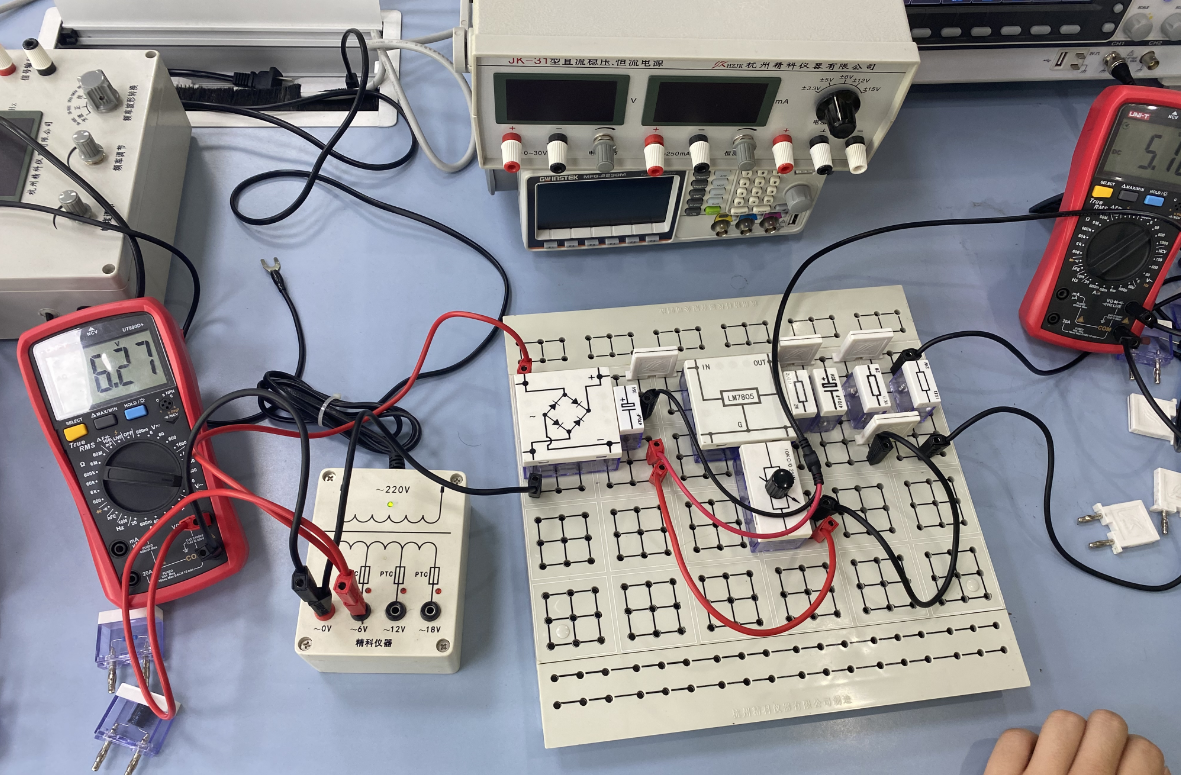
\includegraphics[width=0.6\textwidth]{assets/instruments.png}
    \caption{实验仪器}
\end{figure}

\textbf{三、实验原理}

\textbf{1. 惠斯登电桥}

如图\ref{fig:wheatstone}所示，惠斯登电桥将待测电阻$R_x$与另外2个固定电阻$R_1$、$R_2$和可变电阻$R_0$连接成一个闭路的电阻四边形。电池$E$通过与四边形的两个相对顶端$A$和$B$相连，在另外两个相对顶端$C$和$D$之间接入检流计。

\begin{figure}[H]
    \centering
    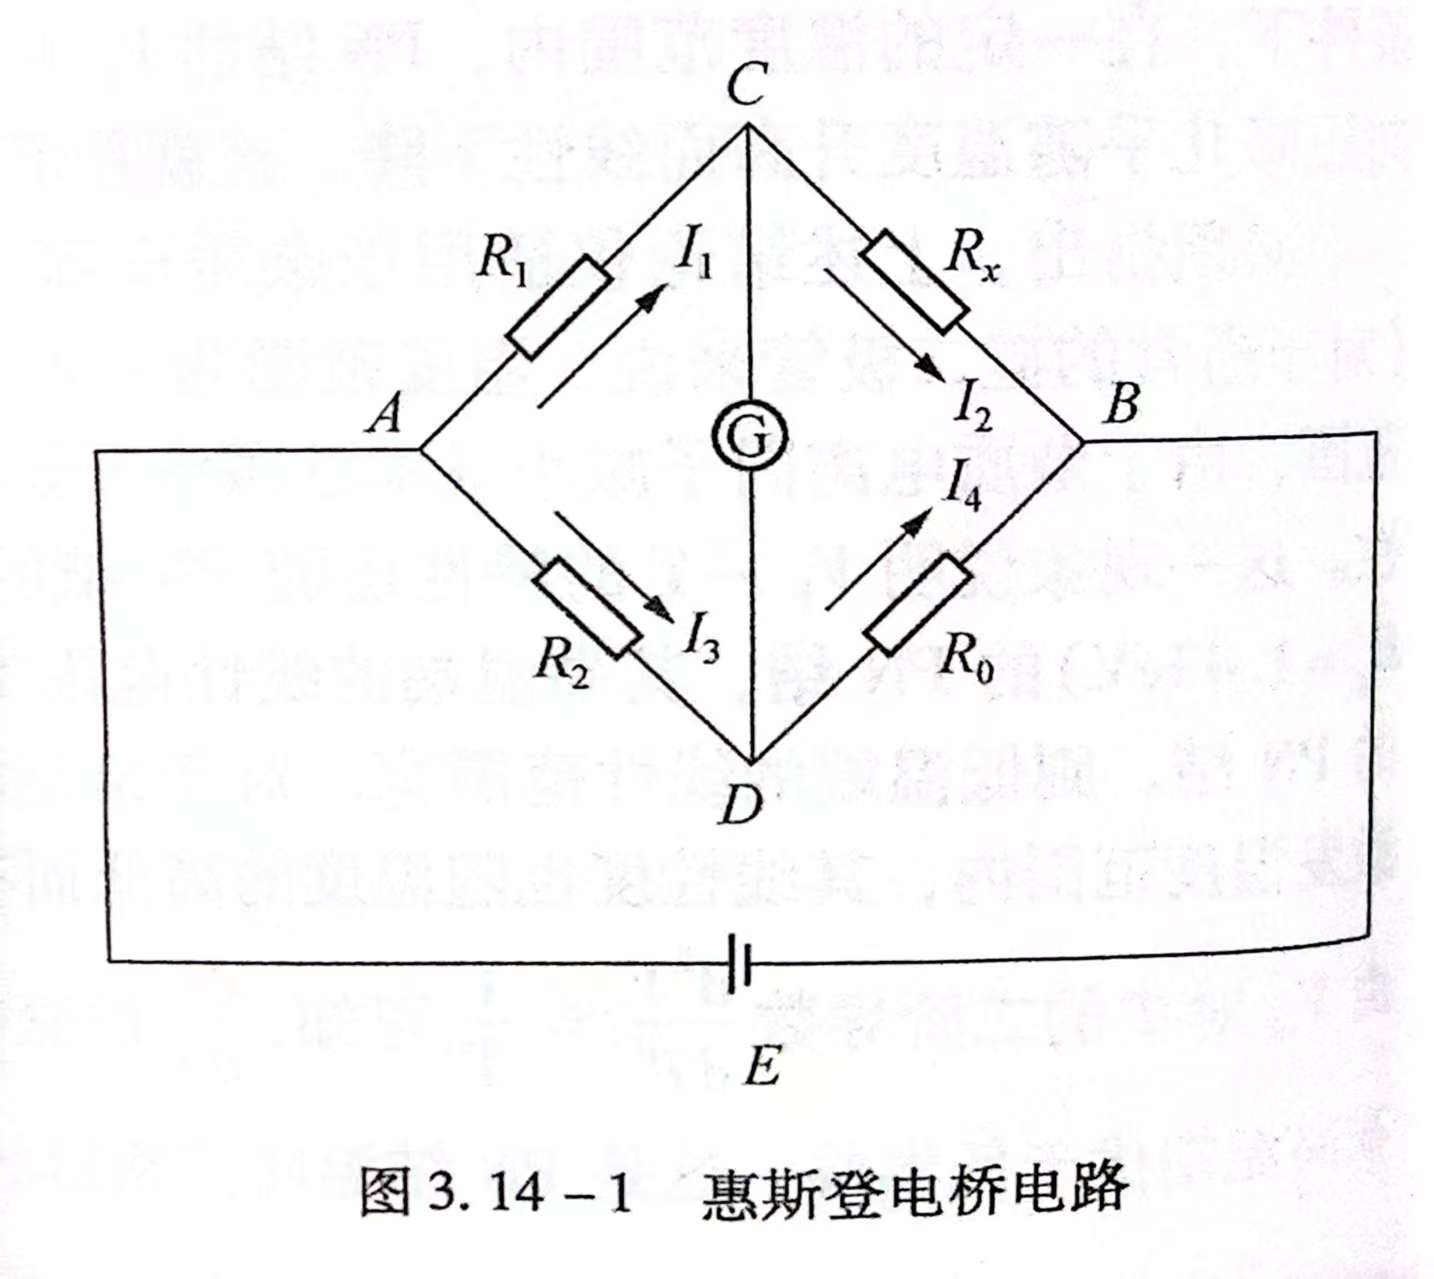
\includegraphics[width=0.5\textwidth]{assets/Wheatstonebridge.jpg}
    \caption{惠斯登电桥电路}
    \label{fig:wheatstone}
\end{figure}

\textbf{2. 平衡条件}

当$C$和$D$两点电位相等时（即$V_{AC} = V_{AD}$），检流计中无电流通过，电桥达到平衡，此时：

\begin{align}
    \frac{R_1}{R_x} = \frac{R_2}{R_0}
\end{align}

即：

\begin{align}
    R_x = \frac{R_1}{R_2}R_0 = KR_0
\end{align}

式中，$K = \frac{R_1}{R_2}$称为比率。若$R_1$、$R_2$、$R_0$（或$K$和$R_0$）为已知，$R_x$即可由上式求出。

\textbf{3. 电桥的灵敏度}

公式$R_x = \frac{R_1}{R_2}R_0 = KR_0$是在电桥平衡条件下的结果，而电桥是否平衡，实际上是通过检流计有无偏转来判断的。本次实验所使用的检流计用万用电表代替，微调时根据数字变化$10^{-6}$ A进行实验。

电桥灵敏度$S$的概念定义为：

\begin{align}
    S = \frac{\Delta n}{\Delta R_x/R_x}
\end{align}

式中，$\Delta R_x$是在电桥平衡后$R_x$的微小改变量（实际上待测电阻$R_x$是不变的，改变的是电阻$R_0$）；$\Delta n$是由于电桥偏离平衡而引起的检流计指针偏转的格数。

$S$越大，说明电桥越灵敏，误差也就越小。在实际中，通常$R_0$是可变的，因此：

\begin{align}
    S = \frac{\Delta n}{\Delta R_0/R_0}
\end{align}

\textbf{4. 电桥的测量误差}

当在符合仪器规定的参考条件下使用时，根据JJQ125-86文件规定，电桥的基本误差极限可用下式表示：

\begin{align}
    E_{lim} = \pm\frac{\alpha}{100}(\frac{R_n}{10} + R_0)k
\end{align}

式中，$\alpha$为电桥的准确度等级；$k$为缩放因子，取电桥的比率；$R_0$为测量盘示值；$R_n$为基准值，各有效量程的基准值应为该量程内最大值的10的整数幂。

一般在实验中由电桥的灵敏度引入的误差$\Delta R$是这样估测的：

在电桥平衡时，将$R_0$改变$\Delta R_0$，使检流计指针偏转的格数$\Delta n = 2$，而人的眼睛观察到的界限是0.2格，所以取：

\begin{align}
    \Delta R = 0.2 \times \frac{\Delta R_0}{2}
\end{align}

测量结果误差可表示为
$$
\sigma_R \approx \sqrt{E_{lim}^2+(\Delta R)^2}
$$

特别的，本次实验使用万用电表代替检流计，因此查看检流计偏转的操作实际为查看电表数字变化。

\textbf{5. 交换测量法（互易法）}

用交换$R_0$和$R_x$的测量法可消除因$R_1$、$R_2$引入的误差，但在保持$R_1/R_2$比值不变的条件下，将$R_0$和$R_x$交换位置，调节$R_0$为$R_0'$，使电桥重新平衡，则：

\begin{align}
    R_x = \sqrt{R_0 \cdot R_0'}
\end{align}

这表明使用交换法可消除由$R_1$、$R_2$引入$R_x$的误差。

\textbf{四、实验步骤}

\textbf{1. 万用表直接测量电阻}

用数字万用表直接测量三个未知电阻$R_{x1}$、$R_{x2}$、$R_{x3}$的阻值，记录测量结果作为参考标准值。使用万用表时，应选择合适的量程，确保测量的准确性。

\textbf{2. 惠斯登电桥测量电阻}

\begin{figure}[H]
    \centering
    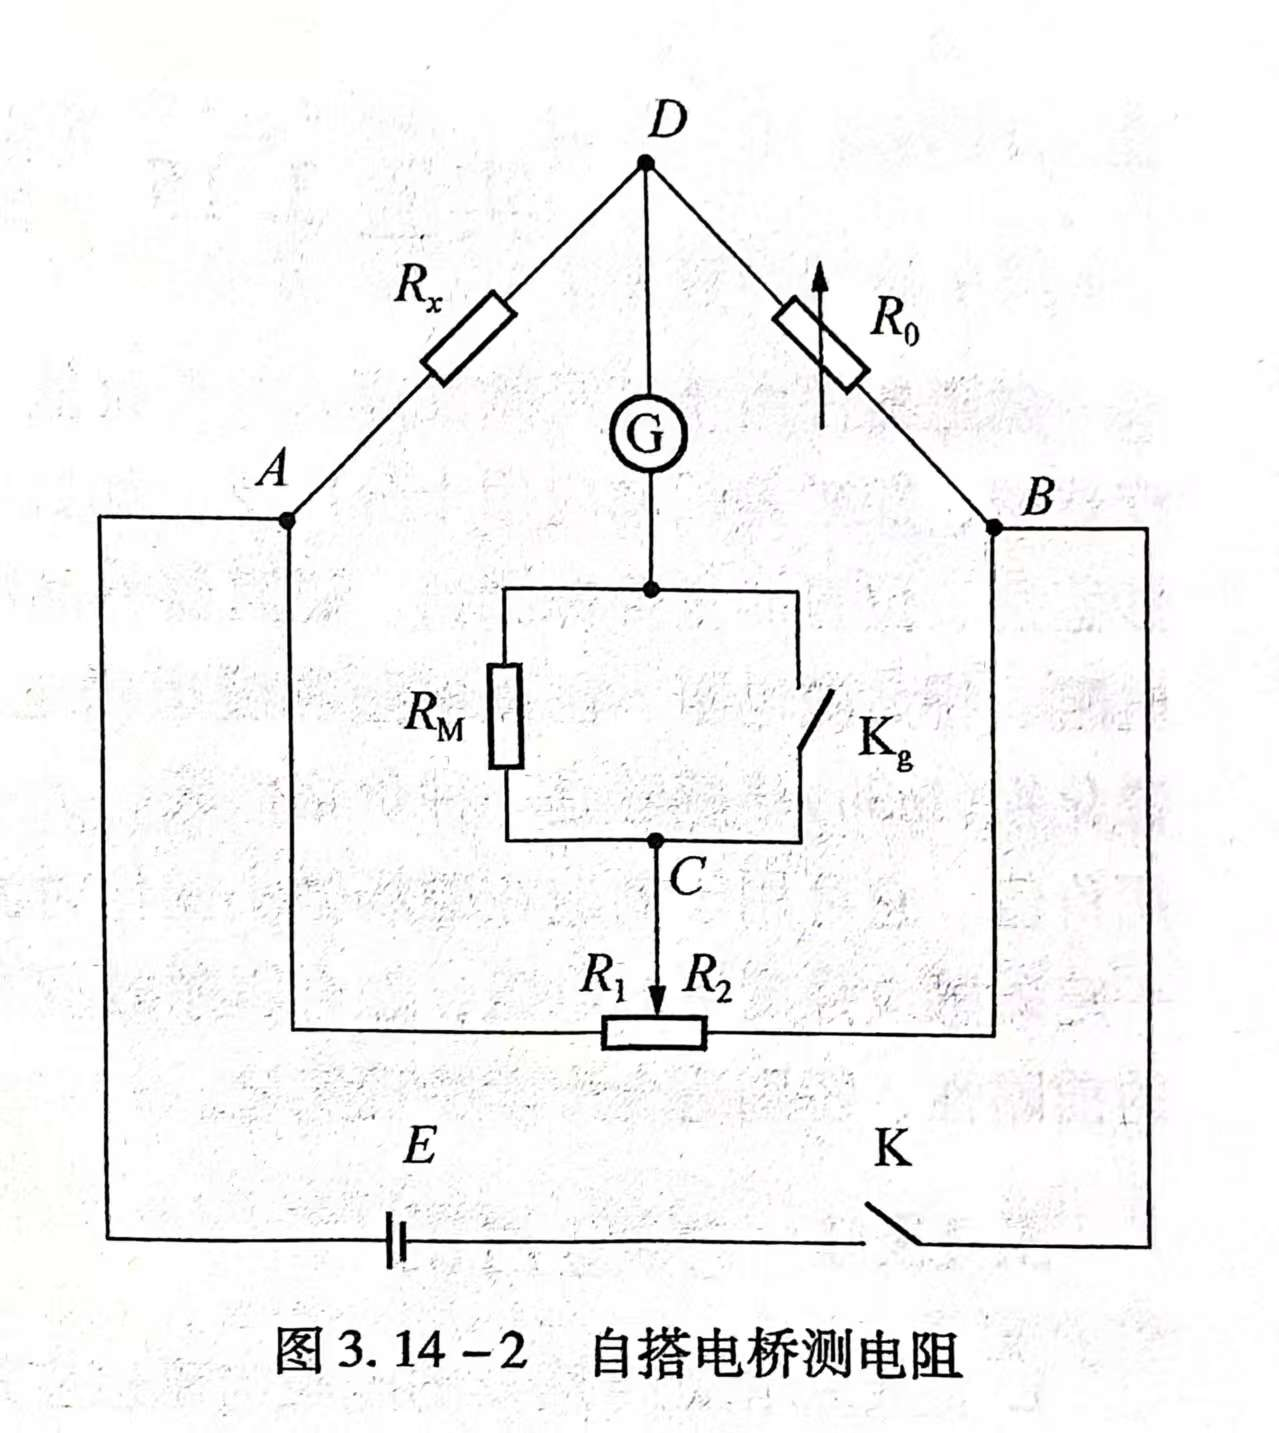
\includegraphics[width=0.5\textwidth]{assets/self_bridge.jpg}
    \caption{自搭电桥测量电路图}
    \label{fig:self_bridge}
\end{figure}

按照图\ref{fig:self_bridge}连接电路，步骤如下：
\begin{enumerate}
    \item 在9孔插件板上搭建电路，$R_M = 10\mathrm{k}\Omega$（保护电阻）
    \item 设置电源电压$E = 5\mathrm{V}$
    \item 将待测电阻$R_x$接入电路
    \item 调节$R_0$使检流计示数为零，电桥达到平衡
    \item 记录此时$R_0$的数值
    \item 轻微调节$R_0$使检流计指示为$+0.1\mu\mathrm{A}$，记录$R_0$值
    \item 调节$R_0$使检流计指示为$-0.1\mu\mathrm{A}$，记录$R_0$值
    \item 记录使检流计偏转$\pm2$格时的$\Delta R_0$值
    \item 根据公式$R_x = \frac{R_1}{R_2}R_0 = KR_0$计算$R_x$（在实验中$K=1$）
\end{enumerate}

\textbf{3. 互易法测量电阻}

\begin{enumerate}
    \item 保持电路和比率臂$R_1/R_2$不变
    \item 记录电桥平衡时$R_0$的值
    \item 交换$R_0$与$R_x$位置，重新调节电桥平衡
    \item 记录新的平衡位置$R_0'$
    \item 调节以获得$\pm0.1\mu\mathrm{A}$时的$R_0'$值
    \item 记录使检流计偏转$\pm2$格时的$\Delta R_0$值
    \item 根据公式$R_x = \sqrt{R_0 \cdot R_0'}$计算$R_x$
\end{enumerate}

此方法可消除因$R_1$、$R_2$不准确引入的系统误差。

\textbf{五、数据处理与结果分析}

\textbf{1. 原始数据}

\textbf{(1) 万用表直接测量电阻}

\begin{table}[H]
    \centering
    \begin{tabular}{|c|c|}
        \hline
        被测电阻 & 万用表测量电阻 \\
        \hline
        $R_{x1}$ & $R_{x1}= 575\Omega$ \\
        \hline
        $R_{x2}$ & $R_{x2}= 471\Omega$ \\
        \hline
        $R_{x3}$ & $R_{x3}= 353.8\Omega$ \\
        \hline
    \end{tabular}
    \caption{万用表测量数据记录}
    \label{tab:multimeter}
\end{table}

\textbf{(2) 惠斯登电桥测量电阻}

\begin{table}[H]
    \centering
    \begin{tabular}{|c|c|c|c|}
        \hline
        \multirow{3}{*}{被测电阻} & \multicolumn{3}{c|}{惠斯登电桥测量电阻} \\
        \cline{2-4}
        & 平衡位置$R_0$ & $+0.1\mu\mathrm{A}$ & $-0.1\mu\mathrm{A}$ \\ 
        \cline{3-4}
        & $(\Omega)$ & $+\Delta R_0 (\Omega)$ & $-\Delta R_0 (\Omega)$ \\ 
        \hline
        $R_{x1}$ & $577.7$ & $0.1$ & $0.1$ \\
        \hline
        $R_{x2}$ & $468.8$ & $0.1$ & $0.1$ \\
        \hline
        $R_{x3}$ & $355.0$ & $0.1$ & $0.1$ \\
        \hline
    \end{tabular}
    \caption{惠斯登电桥测量数据记录}
    \label{tab:wheatstone}
\end{table}

\textbf{(3) 互易法测量电阻}

\begin{table}[H]
    \centering
    \begin{tabular}{|c|c|c|c|c|c|c|}
        \hline
        \multirow{3}{*}{被测电阻} & \multicolumn{6}{c|}{互易法测量电阻} \\
        \cline{2-7}
        & \multicolumn{3}{c|}{原始位置$R_0$} & \multicolumn{3}{c|}{交换后位置$R_0'$} \\
        \cline{2-7}
        & 平衡值 & $+\Delta R_0$ & $-\Delta R_0$ & 平衡值 & $+\Delta R_0$ & $-\Delta R_0$ \\
        \hline
        $R_{x1}$ & $577.7\Omega$ & $0.1\Omega$ & $0.1\Omega$ & $572.6\Omega$ & $0.1\Omega$ & $0.1\Omega$ \\
        \hline
        $R_{x2}$ & $468.8\Omega$ & $0.1\Omega$ & $0.1\Omega$ & $473.1\Omega$ & $0.1\Omega$ & $0.1\Omega$ \\
        \hline
        $R_{x3}$ & $355.0\Omega$ & $0.1\Omega$ & $0.1\Omega$ & $351.8\Omega$ & $0.1\Omega$ & $0.1\Omega$ \\
        \hline
    \end{tabular}
    \caption{互易法测量数据记录}
    \label{tab:interchange}
\end{table}

\textbf{2. 数据处理结果}

\textbf{(1) 惠斯登电桥测量结果}

由于在实验中比率$K = \frac{R_1}{R_2} = 1$，因此待测电阻$R_x = R_0$：

\begin{table}[H]
    \centering
    \begin{tabular}{|c|c|c|c|}
        \hline
        被测电阻 & 平衡位置$R_0 (\Omega)$ & 计算电阻值$R_x (\Omega)$ & 与万用表测量的相对误差 \\
        \hline
        $R_{x1}$ & 577.7 & 577.7 & 0.47\% \\ % 更新
        \hline
        $R_{x2}$ & 468.8 & 468.8 & 0.47\% \\
        \hline
        $R_{x3}$ & 355.0 & 355.0 & 0.34\% \\
        \hline
    \end{tabular}
    \caption{惠斯登电桥测量结果}
    \label{tab:wheatstone_result}
\end{table}

\textbf{(2) 互易法测量结果}

根据交换法公式$R_x = \sqrt{R_0 \cdot R_0'}$，计算电阻值：

\begin{table}[H]
    \centering
    \begin{tabular}{|c|c|c|c|c|}
        \hline
        被测电阻 & 原始$R_0 (\Omega)$ & 交换后$R_0' (\Omega)$ & 计算电阻值$R_x (\Omega)$ & 与万用表测量的相对误差 \\
        \hline
        $R_{x1}$ & 577.7 & 572.6 & 575.08 & 0.01\% \\ % 更新
        \hline
        $R_{x2}$ & 468.8 & 473.1 & 470.96 & 0.01\% \\ % 更新 R_x 和 相对误差 (基于更精确的计算)
        \hline
        $R_{x3}$ & 355.0 & 351.8 & 353.40 & 0.11\% \\ % 更新 R_x 和 相对误差 (基于更精确的计算)
        \hline
    \end{tabular}
    \caption{互易法测量结果}
    \label{tab:interchange_result}
\end{table}

\textbf{六、误差分析}

\textbf{1. 惠斯登电桥测量电阻的误差分析}

惠斯登电桥测量的误差主要来源于两部分：

\textbf{(1) 电桥基本误差}

根据JJQ125-86文件规定：
\begin{align}
    E_{lim} = \pm\frac{\alpha}{100}\left(\frac{R_n}{10} + R_0\right)k
\end{align}

其中，$\alpha$取0.2（优等精度等级），$R_n$取1000$\Omega$（因为电阻都在100-1000$\Omega$范围内），$k=1$。

对于$R_{x1}$（由惠斯登电桥法测得$R_0 = 577.7\Omega$）：
\begin{align}
    E_{lim} = \pm\frac{0.2}{100}\left(\frac{1000}{10} + 577.7\right) \times 1 = \pm\frac{0.2}{100} \times 677.7 = \pm1.3554\Omega \approx \pm1.36\Omega % 更新
\end{align}

\textbf{(2) 平衡判断的误差}

由电桥灵敏度有限引起：
\begin{align}
    \Delta R = 0.2 \times \frac{\Delta R_0}{2} = 0.2 \times \frac{0.1}{2} = 0.01\Omega
\end{align}

其中$\Delta R_0 = 0.1\Omega$是使检流计偏转$\pm2$格的电阻变化量（根据原始数据表）。

\textbf{(3) 总误差}

测量结果总误差可表示为：
\begin{align}
    \sigma_R \approx \sqrt{E_{lim}^2+(\Delta R)^2} = \sqrt{1.3554^2+0.01^2} \approx \sqrt{1.8371 + 0.0001} \approx 1.3554\Omega \approx 1.36\Omega % 更新
\end{align}

相对误差：
\begin{align}
    \frac{\sigma_R}{R_x} \times 100\% = \frac{1.3554\Omega}{577.7\Omega} \times 100\% \approx 0.23\% % 更新
\end{align}

\textbf{2. 互易法测量电阻的误差分析}

互易法测量电阻的误差分析需考虑$R_x = \sqrt{R_0 \cdot R_0'}$中的误差传递。

对于每次测量，类似惠斯登电桥方法，可得$R_0$和$R_0'$的误差$\sigma_{R_0}$和$\sigma_{R_0'}$。

根据误差传递公式，$R_x = \sqrt{R_0 \cdot R_0'}$的相对误差为：
\begin{align}
    \frac{\sigma_{R_x}}{R_x} = \frac{1}{2}\sqrt{\left(\frac{\sigma_{R_0}}{R_0}\right)^2 + \left(\frac{\sigma_{R_0'}}{R_0'}\right)^2}
\end{align}

以$R_{x1}$为例，$R_0 = 577.7\Omega$, $R_0' = 572.6\Omega$。
$\sigma_{R_0} \approx 1.36\Omega$ （由前述惠斯登电桥单次测量误差估算得到）。
对于$R_0' = 572.6\Omega$，$E_{lim}' = \pm\frac{0.2}{100}(\frac{1000}{10} + 572.6) \times 1 \approx \pm1.3452\Omega$。
因此，$\sigma_{R_0'} \approx \sqrt{1.3452^2 + 0.01^2} \approx 1.3452\Omega \approx 1.35\Omega$。

\begin{align}
    \frac{\sigma_{R_x}}{R_x} &= \frac{1}{2}\sqrt{\left(\frac{1.36}{577.7}\right)^2 + \left(\frac{1.35}{572.6}\right)^2} \\ % 更新 R0, R0' sigma_R0, sigma_R0'
    &\approx \frac{1}{2}\sqrt{(0.002354)^2 + (0.002358)^2} \\ % 更新
    &\approx \frac{1}{2}\sqrt{5.542 \times 10^{-6} + 5.560 \times 10^{-6}} \\ % 更新
    &\approx \frac{1}{2}\sqrt{1.1102 \times 10^{-5}} \approx \frac{1}{2} \times 0.003332 \approx 0.00167 % 更新
\end{align}

绝对误差 ($R_x \approx 575.08\Omega$):
\begin{align}
    \sigma_{R_x} = 0.00167 \times 575.08\Omega \approx 0.96\Omega % 更新
\end{align}

相对误差百分比：
\begin{align}
    0.00167 \times 100\% = 0.17\%
\end{align}

互易法测量的误差显著小于惠斯登电桥方法（$0.17\% < 0.23\%$），这验证了交换法在消除系统误差方面的优势。

\textbf{七、结论和讨论}

\textbf{1. 实验结论}

1. 通过万用表直接测量、惠斯登电桥法和交换法（互易法）三种方法测量了三个未知电阻的阻值，结果如下表所示：

\begin{table}[H]
    \centering
    \begin{tabular}{|c|c|c|c|}
        \hline
        被测电阻 & 万用表测量 & 惠斯登电桥法 & 互易法 \\
        \hline
        $R_{x1}$ & $575.0\Omega$ & $577.7\Omega$ & $575.08\Omega$ \\ % 更新
        \hline
        $R_{x2}$ & $471.0\Omega$ & $468.8\Omega$ & $470.96\Omega$ \\ % 更新
        \hline
        $R_{x3}$ & $353.8\Omega$ & $355.0\Omega$ & $353.40\Omega$ \\ % 更新
        \hline
    \end{tabular}
    \caption{三种方法测量结果比较}
    \label{tab:comparison}
\end{table}

2. 惠斯登电桥法测量电阻的相对误差（以$R_{x1}$为例进行的不确定度分析）约为0.23\%，而互易法的相对误差（以$R_{x1}$为例进行的不确定度分析）约为0.17\%，表明互易法可以有效消除因$R_1$、$R_2$不准确引起的系统误差，提高测量精度。

3. 从实验结果看，三种方法测得的电阻值非常接近，最大相对差异（例如$R_{x1}$惠斯登法$577.7\Omega$与万用表$575.0\Omega$相比，差异约为$2.7\Omega$，相对万用表值为$0.47\%$）不超过1\%，表明实验方法可靠，测量结果准确。

\textbf{2. 讨论与改进}

1. 电桥测量中的误差主要来源：
   - 仪器本身的误差
   - 电桥灵敏度有限导致的判断误差
   - $R_1$和$R_2$的不准确性引入的误差（可通过交换法消除）
   - 检流计灵敏度不足
   - 连接线和接触电阻的影响
   - 温度变化对电阻值的影响

2. 为提高测量精度可采取的措施：
   - 使用更高精度的电阻箱和检流计
   - 保持实验环境温度稳定
   - 确保接触良好，减少接触电阻
   - 增加测量次数，取平均值
   - 采用交换法消除系统误差

3. 实验中使用的电桥比率$K=1$，这样可以简化计算，但在实际应用中，应根据被测电阻的大小选择合适的比率，以获得最佳的测量精度。

\textbf{八、思考题解答}

\textbf{1. 交换法测量$R_x$的原理证明}

\begin{proof}
当电桥平衡时，有：
\begin{align}
\frac{R_x}{R_1} = \frac{R_0}{R_2} \Rightarrow \frac{R_x}{R_0} = \frac{R_1}{R_2} \quad (1)
\end{align}

交换$R_0$和$R_x$位置后，再次平衡：
\begin{align}
\frac{R_0'}{R_1} = \frac{R_x}{R_2} \Rightarrow \frac{R_0'}{R_x} = \frac{R_1}{R_2} \quad (2)
\end{align}

由(1)和(2)得：$\frac{R_x}{R_0} = \frac{R_0'}{R_x}$，交叉相乘：
\begin{align}
R_x^2 = R_0 \cdot R_0'
\end{align}

因此：$R_x = \sqrt{R_0 \cdot R_0'}$。
\end{proof}

\textbf{2. 无检流计测量表头内阻}

如果没有检流计，可以用电压测量法测量表头内阻：将电压表接在电桥的C、D两点间，调节$R_0$使电压表示数最小（趋近于零），此时电桥平衡。或者用数字万用表替代检流计，观察电流最小值确定平衡点。

具体步骤如下：
\begin{enumerate}
    \item 将表头作为待测电阻$R_x$接入电桥
    \item 将数字万用表切换至微安电流档，连接至电桥的C、D两点
    \item 调节$R_0$使万用表读数最小（趋近于零）
    \item 记录此时$R_0$值
    \item 可采用交换法再次测量以提高精度
    \item 根据$R_x = R_0$（或$R_x = \sqrt{R_0 \cdot R_0'}$）计算表头内阻
\end{enumerate}

由于表头内阻通常较小，测量时应选择适当的比率$K$，以保证测量精度。

\end{document}
